\section{Shuffle to SAT}

First, we assume that $R_1$ is finite regular language.
This is possible in assumption that the error can usually be detected in the small number of the loops iterations,
so at the first step we can approximate general regular language by finite unrolling of loops.
This assumption is used in bounded model checking~\cite{BMC}.

We should check wheter exists $\omega \in R_1$ such that $\omega \in \mathcal{L}$.
If $\omega$ exists then it should be representable as shuffle of strings $\Omega = \{\omega^i | \omega^i \in L_i, i\in 1 \dots n\}$.
Our procedure trys to finde such $\Omega$, so if our system can demonstrate bad behavior then we will not only detect this fact, but also provide an ``trace'' for each function which may be useful for results understanding.

The first step is creation of the regular language $R_2$ of all possible subsequnces of $R_1$: $R_2 = \{ v_1 \dots v_k | \exists \{u_i| u_i \in \Sigma^* \}_{i\in 0 \dots k+1} (u_0 v_1 u_1 \dots v_k u_{k+1} \in R_1) \}$.
It can be done, for example, by adding new edges in DFA $M_1$ which represents $R_1$: $E(M_2)=E(M_1) \cup \{(v_i,l_i,v_j) | (v_k,l_i,v_j) \in E(M_1) \text{ and } v_k $ is reachable from $ v_i \text{ in } M_1\}$.
In this step we should suppose that all symbols are unique.
It is necessary for futher steps and may be done, for example, by extending symbol with its position.
Note that $|V(M_2)| = |V(M_1)|$ and $|E(M_2)| = O(|V(M_1)|^2)$.

The next step is a calculation of $\Omega' = \bigcup\limits_{i\in 1 \dots n} L_{f_i} \cap R_2$.
It is well-known that intersection of context-free language with regular one is a context-free language.
Practical aspects of such intersection construction is actively 
We use an algorithm described in paper~\cite{Grigorev} because it provide useful representation of intersection result.
This algorithm is based on Generalised LL (GLL)~\cite{scott2010gll} and utilizes the Binarized Shared Packed Parse Forest (SPPF)~\cite{brnglr, SPPF} for result representation.
Binarized SPPF compresses derivation trees optimally reusing common nodes and subtrees, thus utilizing it for parsing forest representation grants worst-case cubic space complexity~\cite{scott2010gll} which allows us to get compact formula for SAT-solver.

Binarized SPPF can be represented as a graph in which each node has one of four types described below.
We denote the start and the end positions of substring as $i$ and $j$ respectively, and we call tuple $(i,j)$ an \textit{extension} of a node.

\begin{itemize}
    \item \textbf{Terminal node} with label $(i, T, j)$.
    \item \textbf{Nonterminal node} with label $(i, N, j)$. 
    This node denotes that there is at least one derivation for substring $\alpha=\omega[i..j-1]$ such that $N \Rightarrow^*_G \alpha, \alpha = \omega[i..j-1] $.
    All derivation trees for the given substring and nonterminal can be extracted from SPPF by left-to-right top-down graph traversal started from respective node.     
    \item \textbf{Intermediate node}: a special kind of node used for binarization of SPPF. These nodes are labeled with $(i,t,j)$, where $t$ is a grammar slot.
    \item \textbf{Packed node} with label $(N \rightarrow \alpha, k)$. 
    Subgraph with ``root'' in such node is one possible derivation from nonterminal $N$ in case when the parent is a nonterminal node labeled with $(<\mkern-9mu | \mkern-9mu> (i, N, j))$.
    
\end{itemize}

The $\Omega'$ is closed to $\Omega$ but we should additionally guarantee, that each symbol uses only ones through all strings.
It is required for shuffle and will be done at the next step.


!!!!!!. This fomula 
can be built via recursive traversal of SPPF. We convert the binary nodes to the conjunction of children, or in case of multiple 
derivations --- alternation. Terminal nodes of the form ($i,a_i,j$) of $m$'th SPPF are to be transformed to bool
variables $(ia_i^mj)$.

In addition to conjunction of formulas describing SPPFs, there are needed an expression to preserve the
shuffle semantics: the terminals .... should be cosen exactly once, this grants the fact that the union of strings results a valid 
path in $R_1$. For the one path $a b c ...$ in $R_1$ and $n$ given SPPFs the formula describing such condition is a 
conjunction of parts $(1a^1 2)\ XOR\ (1a^2 2)\ XOR\ (1a^3 2)\ ...\ (1a^n 2) $ for each terminal.


To demonstrate an example of formula generation we consider a shuffle of 2 languages 
produced by grammars $G_1: A\rightarrow K\ c;\ K \rightarrow a\ b\ |\ x\ a$ % $G_1: A\rightarrow K\ c;\ K \rightarrow a\ b\ |\ 1\ a$
and $G_2: B \rightarrow x\ y\ z$ %$G_2: B \rightarrow 1\ 2\ 3$
. $A$ and $B$ are start nonterminals.
We want to check for emptiness an intersection of this shuffle with a string $1ab2c3$. 
A finite automaton for transitive closure of this trace shown below.

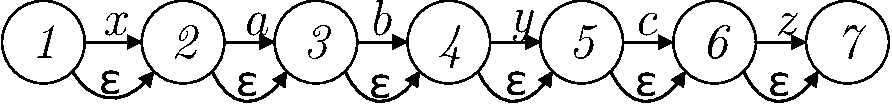
\includegraphics[scale=.54]{./pic/trace2.pdf}

The results of the intersection of languages defined by $G_1$ and $G_2$ are presented as SPPFs in picture
below. Black dots are packed nodes. Note that we removed redundant intermediate and packed nodes from the 
SPPFs to simplify them and to decrease the size of the structure.

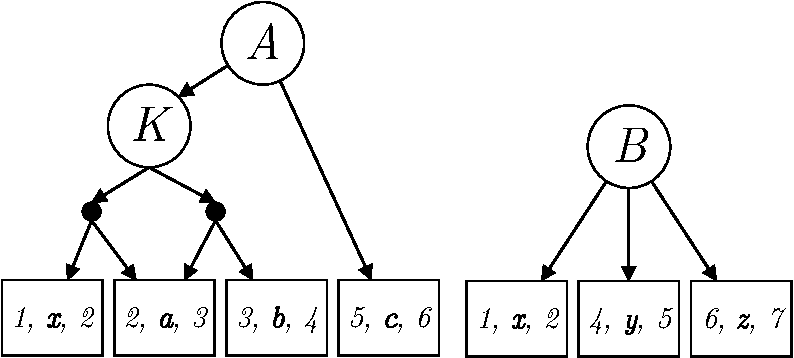
\includegraphics[scale=.6]{./pic/trees2.pdf}


We generate formula $F_1 = (1 x^1 2\ \&\ 2 a^1 3\ |\ 2 a^1 3\ \&\ 3 b^1 4)\ \&\ 5 c^1 6$  % $F_1 = (1 1^1 2\ \&\ 2 a^1 3\ |\ 2 a^1 3\ \&\ 3 b^1 4)\ \&\ 5 c^1 6$ 
for the SPPF for grammar $G_1$
and formula $F_2 = \ 1 x^2 2\ \&\ 4 y^2 5\ \&\ 6 z^1 7$ %$F_2 = \ 1 1^2 2\ \&\ 4 2^2 5\ \&\ 6 3^1 7$
for the second SPPF. Conditions for the 
terminals are described by $F_3 = \ (1 x^1 2\ XOR\ 1 x^2 2)\ \&\ (2 a^1 3\ XOR\ 2 a^2 3)\ \&\ ...\ \&\ (6 z^1 7\ XOR\ 6 z^2 7)$.
%$F_3 = \ (1 1^1 2\ XOR\ 1 1^2 2)\ \&\ (2 a^1 3\ XOR\ 2 a^2 3)\ \&\ ...\ \&\ (6 3^1 7\ XOR\ 6 3^2 7)$.
The final SAT problem is $F_1\&F_2\&F_3$.
